\chapter{Zadanie 1}
	\label{ch:z1}
	\section{Implementacja i analiza modelu obiektu}
	\label{sec:model}
		W celu zaimplementowania obiektu w programie Matlab potrzebna była postać dyskretna opisujących go równań. Dla wyznaczenia wzoru dyskretnego pochodnej zdecydowaliśmy się na okres próbkowania równy 1s. Otrzymane po dyskretyzacji i przekształceniach wzory wyglądają następująco:
	
		\begin{equation}
			\left\{
			\begin{tabular}{l}
				$V_1(k) =V_1(k-1) + F_1(k-1) + F_D(k-1) - \alpha_1\sqrt{h_1(k-1)}$ \\\\
				$V_2(k) = V_2(k-1)+\alpha_1\sqrt{h_1(k-1)} - \alpha_2\sqrt{h_2(k-1)}$\\\\
				$h_1(k) = \sqrt{\frac{V_1(k)}{C_1}}$\\\\
				$h_2(k) = \sqrt{\frac{V_2(k)}{C_2}}$\\\\
				$F_1(k) = F_{1in}(k-50)$
			\end{tabular}
			\right.
			\label{eq:dyskretne}
		\end{equation}
	
		W celu zanalizowania modelu obiektu przeprowadzone zostało badanie reakcji wyjścia $h_2$ na skok sterowania $F_{1in}$ oraz zakłócenia $F_D$. Skoki zostały przeprowadzone w chwili t = 60s. Skoki wykonywane były startując z podanego punktu pracy dla wartości od 24 do 84 co 10 dla sterowania oraz od 5 do 15 co 2.5 dla zakłócenia. Otrzymane wyniki przedstawione zostały na wykresach \ref{rys:model_u} oraz \ref{rys:model_z}. Jak widać z wykresu dla zmiennego sterowania obiekt z całą pewnością nie jest liniowy. Już przy zmianie sterowania z 54 na 64 różnica wartości wyjścia jest widocznie większa niż przy zmianie z 54 na 44. Porównując przebiegi dla różnych wartości skoków możemy stwierdzić, że przy zwiększaniu sterowania obiekt staje się coraz łagodniejszy, ale różnica w wartości wyjścia zwiększa się. Dla mniejszych sterowań wynik jest odwrotny. Dla zmian zakłócenia obiekt także jest nieliniowy, jednakże różnica między przebiegami dla tak małych zmian jest niemalże niezauważalna. Na wykresach widać także wpływ opóźnienia sterowania $F_{1in}$ względem wejścia $F_1$. Zmiany wartości sterowania spotykają się z opóźnioną reakcją obiektu, w przeciwieństwie do zmian zakłócenia.
		
		\begin{figure}
			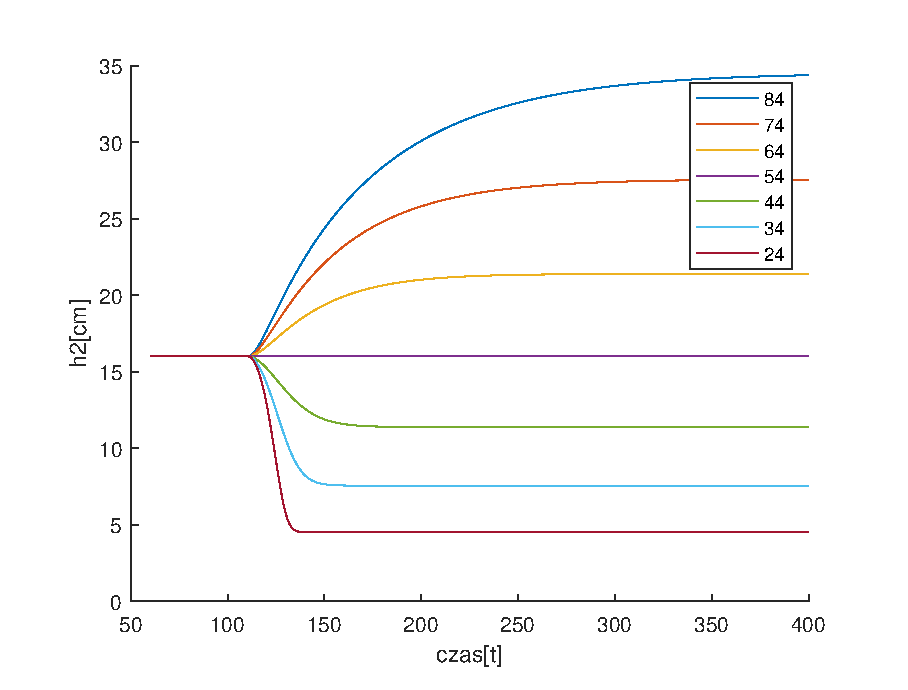
\includegraphics[width=0.9\linewidth]{plots/z1_model_u.eps}
			\caption{Przebiegi wyjścia dla skoku wartości sterowania w chwili 60s}
			\label{rys:model_u}
		\end{figure}
		\begin{figure}
			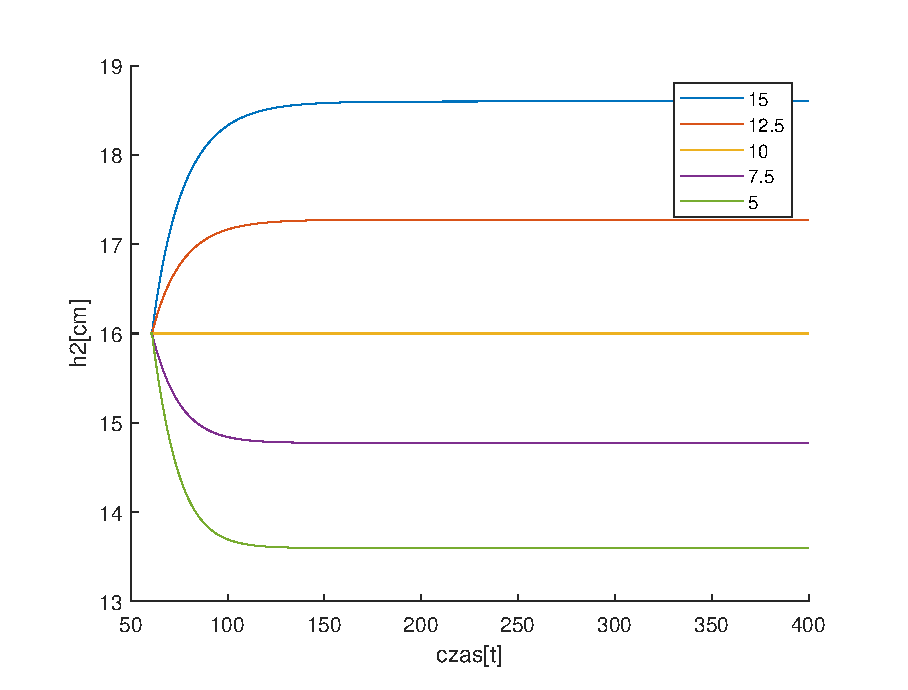
\includegraphics[width=0.9\linewidth]{plots/z1_model_z.eps}
			\caption{Przebiegi wyjścia dla skoku wartości sterowania w chwili 60s}
			\label{rys:model_z}
		\end{figure}
		\newpage

	\section{Model liniowy}
		\label{sec:model_lin}
		W celu uzyskania modelu liniowego należy zlinearyzować równania obiektu w podanym punkcie pracy. Zlinearyzowane równania wyglądają następująco:
		\begin{equation}
			\left\{
			\begin{tabular}{l}
				$V_1(k) =V_1(k-1) + (F_1(k-1)-F_{10}) + (F_D(k-1)-F_{D0}) -\frac{\alpha_1}{2\sqrt{h_{10}}}*(h_1(k-1)-h_{10}) $ \\\\
				$V_2(k) = V_2(k-1)+\frac{\alpha_1}{2\sqrt{h_{10}}}*(h_1(k-1)-h_{10}) - \frac{\alpha_2}{2\sqrt{h_{20}}}*(h_2(k-1)-h_{20})$\\\\
				$h_1(k) = h_{10}+\frac{1}{2\sqrt{C_1*V_{10}}}*(V_1(k)-V_{10})$\\\\
				$h_2(k) = h_{20}+\frac{1}{2\sqrt{C_2*V_{20}}}*(V_2(k)-V_{20})$\\\\
				$F_1(k) = F_{1in}(k-50)$
			\end{tabular}
			\right.
			\label{eq:lin}
		\end{equation}
		
		O ile $F_{10}$, $F_{D0}$ oraz $h_{10}$ mamy podane, tak $V_{10}$, $V_{20}$ oraz $h_{10}$ musimy sobie określić. Nie jest to złożone zadanie. W punkcie pracy pochodne obydwu objętości musi być zerowa, z czego wynika, że $F_2 = F_3 => \alpha_1*\sqrt{h_1} = \alpha_2*\sqrt{h_2}$. Ponieważ $\alpha_1 = \alpha_2$ to wysokość wody w punkcie pracy musi być taka sama dla obydwu zbiorników. Mając wysokości wody w obu zbiornikach można obliczyć jej objętość.
		
		Dla uzyskanego w ten sposób modelu liniowego przeprowadzono takie same testy jak dla oryginalnego modelu. Wynik testów przedstawiony jest na wykresach \ref{rys:modellin_u} oraz \ref{rys:modellin_z}, na których niebieskim kolorem widnieją przebiegi oryginalne, a różowym te dla obiektu zlinearyzowanego. Dla skoków sterowania do 44 oraz 64 przebiegi dla obydwu modeli są dosyć podobne zarówno kształtem jak i wartościami. Dla wysokich oraz niskich wartości nie jest już niestety tak dobrze. Obiekt liniowy ,w przeciwieństwie do oryginału, działa z taką samą dynamiką dla całego zakresu, co oznacza, że dla wysokich wartości sterowania jest on od niego szybszy, a dla niskich wolniejszy. Co więcej im dalej od punktu pracy tym większa różnica w wartości końcowej wyjścia. Dla skoków zakłócenia osiągane wartości są zbliżone dla skoków do 7.5 i 12.5. Niższe oraz wyższe spadki powodują coraz większe odchylenie końcowej wartości wyjścia, choć i tak wciąż nie jest ono bardzo duże. Jeśli chodzi o dynamikę obiekt zlinearyzowany reaguje na zmianę zakłócenia nieco wolniej niż obiekt oryginalny.
		
		\begin{figure}
			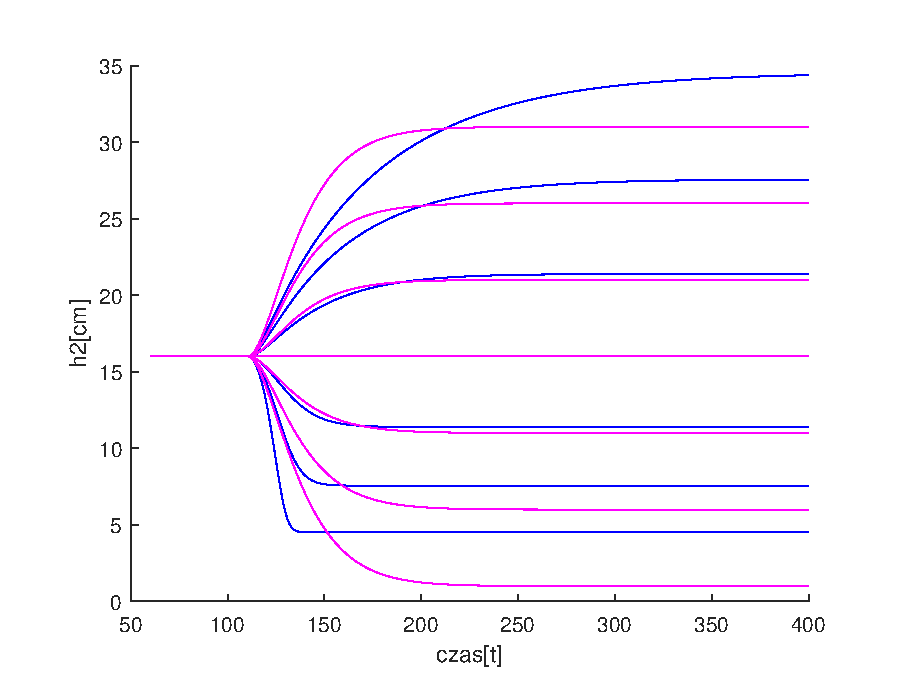
\includegraphics[width=0.9\linewidth]{plots/z1_modellin_u.eps}
			\caption{Przebiegi wyjścia dla skoku wartości sterowania w chwili 60s, dla modelu nieliniowego i liniowego}
			\label{rys:modellin_u}
		\end{figure}
		\begin{figure}
			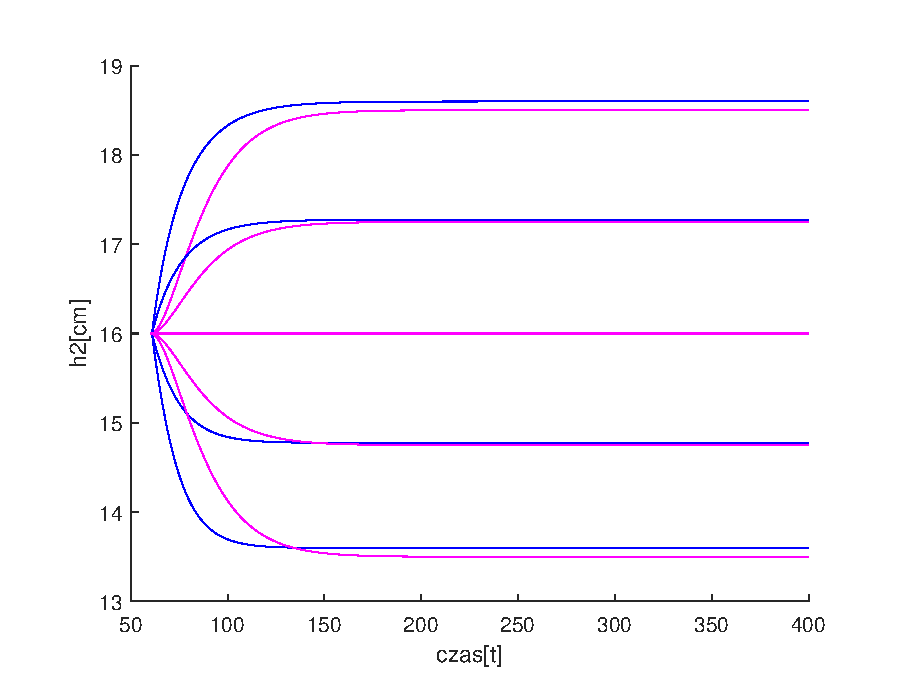
\includegraphics[width=0.9\linewidth]{plots/z1_modellin_z.eps}
			\caption{Przebiegi wyjścia dla skoku wartości sterowania w chwili 60s, dla modelu nieliniowego i liniowego}
			\label{rys:modellin_z}
		\end{figure}
		\newpage